%!TEX root = ../documentation.tex
\chapter{Ergebnisse}
\label{ch:results}

Da dann alles vollendet ist, sowohl das bearbeiten des Datensatzes, als auch das Trainieren der Modelle, bekommt man die ersten Ergebnisse für beide Modelle.

\section{ResNet152}

ResNet152 war das erste geteste Modell, so dass man bei den ersten Ergebnissen geringere Genauigkeiten als erwartet bekommt, jedoch ließ sich das alles beheben indem man sowohl das Training, als auch die Augmentation immer wieder etwas angepasst und verglichen hat. Nach vielen Vergleichen, mit welchen Einstellungen man das beste Ergebnis bekommt, haben wir die Finale folgende Confusion Matrix (Abbildung 7.1) erhalten. Hierbei benutzen wir für unser bestes Ergebnis soweit eine Adam Lernrate von 0.01 und decay = 1e-5, den ImageNet weight transfer, Batchgröße von 256 und Bildgröße von 224x224.

\begin{figure}[H]
    \centering
    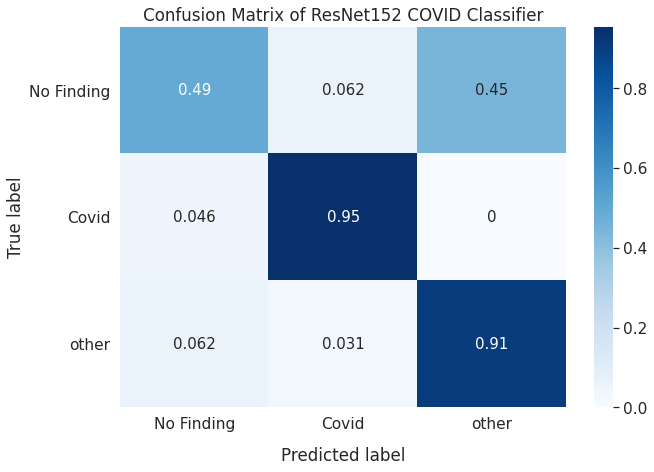
\includegraphics[width=0.75\textwidth]{../results/ResNet152_conf_matrix.png}
    \caption{}
\end{figure}

Hier erkennt man ein mittelmäßig gutes Ergebnis für die Prediction von Covid. Die Genauigkeit liegt bei 78\% (auf unbekannten Daten). Hiermit kann man gut weiter arbeiten und die Schwächen versuchen heraus zu filtern. Vorallem auffällig ist, das Schwanken der Ergebnisse, wenn man sich die gesunden Fälle anguckt, da vorallem die binären Ergebnisse (Covid / kein Covid) für uns relevant sind. Da das Ergebnis für uns dort an einem Maximum angekommen ist, welches durch das binäre Klassifizieren nicht besser wurde, ist es Zeit dieses Modell mit weiteren Modellen zu vergleichen und eventuelle Probleme zu erkennen.

\section{SqueezeNet}

Hier haben wir den Vorteil, dadurch, dass wir bereits ein Modell getestet haben, können wir den Datensatz besser modifizieren und somit effizienter vergleichen.
Hierfür haben wir den Adam Optimizer mit eine Lernrate von 0.0001 (zuvor 0.01). Die Batchgröße wurde deutlich verringer, die Bildergröße vergrößert,um den Vergleich gut sehen zu können. Nach dem dann gegebene Fehler behoben wurden, bekommt man auch hier eine Confusion Matrix für die Ergebnisse (Abbildung 7.2).

\begin{figure}[H]
    \centering
    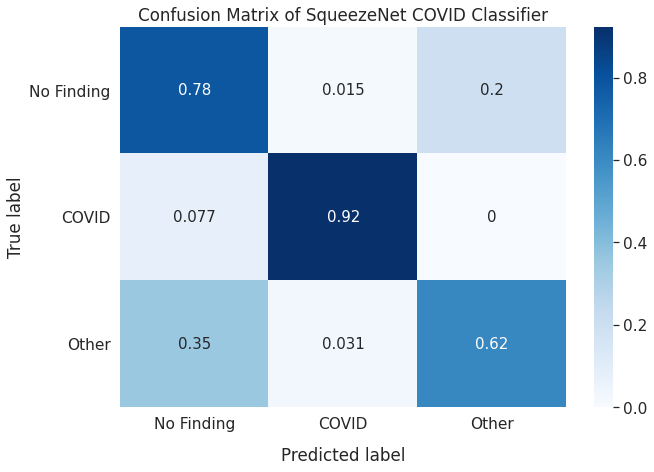
\includegraphics[width=0.75\textwidth]{../results/SqueezeNet_conf_matrix.png}
    \caption{}
\end{figure}

Hier haben wir wieder einen hohen Genauigkeitswert für die richtige Vorhersage von Covid. Im Vergleich zu ResNet152 ist die Genauigkeit von anderen Krankheiten zwar geringer (welche in diesem speziellen Fall für uns nicht weit von Bedeutung sind), die Genauigkeit für die gesunden Patienten jedoch um einiges höher. Die Genauigkeit liegt dann umgerechnet insgesamt bei etwa 77\%. Da die Werte so enger bei einander liegen und so verteilt sind, dass wir die Werte haben, mit denen wir weiter arbeiten möchten, können wir das dann mit der Binären Klassifizierung (Covid / kein Covid) vergleichen, da dieser Test das Hauptziel bei der Bekämpfung von Covid-19 ist. Dort haben wir dann jedoch das optimale Ergebnis mit einer Batchgröße von 64 und einer Bildgröße von 320x320 erreicht (welches bei den vorherigen Ergebnissen nicht viel verändert hat). Die Passende Confusion Matrix sieht man folgend (Abbildung 7.3).

\begin{figure}[H]
    \centering
    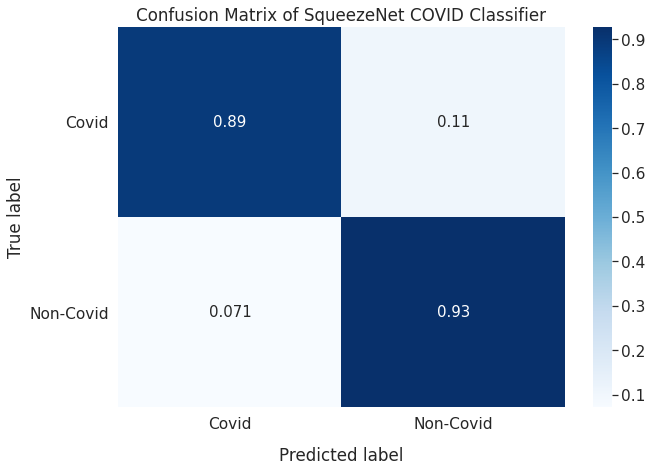
\includegraphics[width=0.75\textwidth]{../results/Binary_SqueezeNet_conf_matrix.png}
    \caption{}
\end{figure}

Bei der binären Klassifizierung erreichen wir für das richtige Vorhersagen von Covid etwa 89\% und für gesunde Patienten etwa 93\%. Rechnet man dies um kommt man auf eine insgesammte Genauigkeit von etwa 92\%, mit welcher SqueezeNet, anhand einer Röntgenaufnahme der Lunge, vorher sagt, ob ein Patient an Covid-19 erkrankt ist oder nicht. Somit haben wir hier mit Abstand das beste Ergebnis bis zum jetzigen Zeitpunkt, welches man bestimmt nach vielen weiteren Experimenten und einem größeren Datensatz noch verbessern kann, aber für uns gut zum weiter arbeiten und vorallem eine gute Feststellung ist, dass man dieses Modell gut trainieren kann, um Covid effizient zu diagnostizieren.